
\documentclass[runningheads]{llncs}
\makeatletter
\AtBeginDocument{%
  \def\doi#1{\url{https://doi.org/#1}}}
\makeatother

%\documentclass[11pt,a4paper]{article} %UKenglish,
%\textheight24cm
%\textwidth16cm
%\topmargin-5mm
%\oddsidemargin0cm
%\evensidemargin0cm

\usepackage{enumerate}
\usepackage{textcomp}
\usepackage{url}
\usepackage{graphicx}
\usepackage{amssymb}
\usepackage{amsmath}
\usepackage{proof}
%\usepackage{amsthm}
\usepackage{verbatim}
%\usepackage{subcaption}
\usepackage[utf8]{inputenc}
%\usepackage[russian]{babel}
\usepackage{color}


\newcommand{\ifdraft}[1]{#1}
\definecolor{aocolour}{rgb}{0.7,0.8,1}
\definecolor{lavender}{rgb}{0.8,0.6,1}
\newcommand{\ao}[1]{\ifdraft{\noindent\colorbox{aocolour}{A.O.: #1}}}
\newcommand{\es}[1]{\ifdraft{\noindent\colorbox{lavender}{E.S.: #1}}}

\newcommand{\xra}[1]{\overset{#1}{\rightsquigarrow}}

\newcommand{\set}[2]{\{ \, #1 \mid #2 \, \}}
\newcommand{\setbig}[2]{\big\{ \: #1 \;\big|\; #2 \: \big\}}
\renewcommand{\emptyset}{\varnothing}
\renewcommand{\epsilon}{\varepsilon}

\newcommand{\itm}[2]{#1(#2)}
\newcommand{\gap}[2]{#1\,{:}\,#2}
\newcommand{\itmcond}[4]{\frac{#1}{#2}(\gap{#3}{#4})}
\newcommand{\ntcondold}[3]{\frac{#1}{#2/#3}}
\newcommand{\ntcond}[4]{\frac{#1/#3}{#2/#4}}
\newcommand{\ntskippedcond}[2]{\ntcond{#1}{#2}{\ldots}{\ldots}}
\newcommand{\ranksymb}{\mathop{\mathrm{rank}}}
\newcommand{\rank}[1]{\ranksymb #1}

\DeclareMathOperator{\osc}{\textup{osc}}

%\newtheorem{lemma}{Lemma}
%\newtheorem{theorem}{Theorem}
%\newtheorem{definition}{Definition}
%\newtheorem{example}{Example}
%\newtheorem{corollary}{Corollary}


\begin{document}

\sloppy

\title{Rational index of languages defined by grammars with bounded dimension of parse trees\thanks{%
	Research supported by the Russian Science Foundation, project 18-11-00100.}
}
\titlerunning{Rational index for grammars with bounded dimension of trees}

\author{Ekaterina Shemetova\inst{1,3}\orcidID{0000-0002-1577-8347}
\and
Alexander Okhotin\inst{1}\orcidID{0000-0002-1615-2725}
\and
Semyon Grigorev\inst{2}\orcidID{0000-0002-7966-0698}
}

\institute{%
	Department of Mathematics and Computer Science,
	St. Petersburg State University, 
	14th Line V. O., 29, Saint Petersburg 199178, Russia
\\ \email{alexander.okhotin@spbu.ru}
\and
	Department of Mathematics and Mechanics,
	St. Petersburg State University, 
	7/9 Universitetskaya nab., Saint Petersburg 199034, Russia
\\ \email{semyon.grigorev@spbu.ru}
\and
	St. Petersburg Academic University, 
	ul. Khlopina, 8, Saint Petersburg 194021, Russia
\\ \email{katyacyfra@gmail.com}
}



\maketitle


\begin{abstract}
The rational index $\rho_L$ of a language $L$ is an integer function,
where $\rho_L(n)$ is the maximum length of the shortest string in $L \cap R$,
over all regular languages $R$ recognized by $n$-state nondeterministic finite automata (NFA).
This paper investigates the rational index of languages
defined by grammars with bounded tree dimension,
and shows that it is polynomial in $n$.
More precisely, it is proved that for a context-free grammar with tree dimension bounded by $d$,
its rational index is at most $O(n^{2d})$,
and that this estimation is asymptotically tight,
as there exists a grammar with rational index $\Theta(n^{2d})$.
For a multi-component grammar of rank $k$ and with tree dimension bounded by $d$,
the rational index is bounded by $O(n^{2kd})$,
and there exists a grammar with rational index $\Omega(n^{2kd})$.

\textbf{Keywords.}
Dimension of a parse tree; Strahler number; rational index; context-free grammars; multiple context-free grammars.
\end{abstract}





\section{Introduction}\label{section_introduction}

The notion of a rational index of a language
was introduced by Boasson, Courcelle and Nivat~\cite{RatBasic}
as a complexity measure for context-free languages.
The rational index $\rho_L$ of a language $L$ is an integer function,
where $\rho_L(n)$ is the maximum length of the shortest string in a language of the form $L \cap R$,
where $R$ is a regular language recognized by an $n$-state nondeterministic finite automaton (NFA),
and the maximum is taken over all such languages $R$ with $L \cap R \neq \emptyset$.

Besides its theoretical value as a measure of complexity of a language,
the rational index is useful
in determining the parallel complexity of practical problems,
such as the CFL-reachability problem
and the more general Datalog query evaluation.
The \emph{CFL-reachability problem} is stated as follows:
for a context-free grammar $G$
given an NFA $A$ over the same alphabet,
determine whether $L(G) \cap L(A)$ is non-empty.
With $A$ regarded as a labelled graph,
%a directed edge-labeled graph $D$ and a pair of nodes $u$ and $v$,
%determine whether there is a path from $u$ to $v$ labeled with a string in $L(G)$.
%That is, CFL-reachability 
this is a kind of graph reachability problem
with path constraints defined by a context-free grammar.
This is an important problem used in static code analysis~\cite{RepsBasic}
and graph database query evaluation~\cite{Yannakakis}.

%Unlike context-free language recognition,
%which is in NC for a fixed context-free grammar,
The CFL-reachability problem is P-complete
already for a fixed context-free grammar~\cite{PCompl}.
%Practically, it means that there is no efficient parallel algorithm
%for solving this problem (unless P $\neq$ NC). 
The question on the parallel complexity of this problem
was investigated by Ullman and Van Gelder \cite{Ullman}
in a much more general case,
with a rich logic for database queries instead of grammars,
and it was proved that under
an assumption called the \emph{polynomial fringe property}
the problem is decidable in NC~\cite{Ullman}.
In the special case of grammars,
the result of Ullman and Van Gelder \cite{Ullman}
gives an NC$^2$ algorithm for the CFL-reachability problem,
under the assumption that the grammar's rational index is polynomial.
% implicit in Corollary 7.1.

%was extensively investigated by the deductive database community~\cite{ChainQ,Ullman}.
%that if the context-free language has a polynomial rational index
%The polynomial fringe property is equivalent to having the polynomial rational index:
%for a context-free language $L(G)$ having the polynomial rational index $\rho_L(n) = poly(n)$,
%where $poly(n)$ is some polynomial, is the same as for corresponding chain query
%to have the polynomial fringe property.

%This motivates further study of
Theoretical properties of the rational index
have received some attention in the literature.
Pierre and Farinone~\cite{GreibRat} proved that for every algebraic number $\gamma \geqslant 1$,
there is a context-free grammar with a rational index of the order $\Theta(n^\gamma)$.
An upper bound on the rational index of a context-free language,
shown by Pierre~\cite{CFRat}, is $2^{\Theta(n^2/\ln n)}$,
and this bound is reached on the Dyck language on two pairs of parentheses.
For several important subfamilies of grammars,
such as the linear and the one-counter languages,
there are polynomial upper bounds on the rational index,
which imply that the CFL-reachability problem is in NC$^2$;
they can be proved to lie in NL
by direct methods not involving the rational index~\cite{labelledGraphs,LReach}.

Other problems on the length of shortest strings
have received some attention in literature.
Chistikov et al.~\cite{ChistikovCzerwinskiHofmanPilipczukWehar}
investigated the length of shortest strings in \emph{one-counter languages},
and, in particular, proved that their rational index is $O(n^2)$.
Ellul et al.~\cite{EllulKrawetzShallitWang} studied the length of the shortest string 
which is not accepted by an NFA. 
Alpoge et al.~\cite{AlpogeAngSchaefferShallit} 
found upper and lower bounds on the length of shortest strings
in regular languages specified in various ways.
The maximum length of shortest strings
for deterministic two-way finite automata (2DFA) 
has been investigated in some recent papers~\cite{DobronravovDobronravovOkhotin,KrymskiOkhotin,MartynovaOkhotin}.

This paper investigates the rational index
of a generalization of linear languages:
the \emph{languages of bounded tree dimension},
that is, those defined by context-free grammars
with a certain limit on branching in the parse trees.
The notion of tree dimension is well-known in the literature,
and appears under different names:
Chytil and Monien~\cite{ChytilMonien} use the term \emph{$k$-caterpillar trees},
Lohrey et al.~\cite{Lohrey22} call this \emph{Horton--Strahler number}, 
Esparza et al.~\cite{EsparzaLuttenbergerSchlund} use the term \emph{Strahler number} of a tree
and mention numerous applications and alternative names for this notion,
while Luttenberger and Schlund~\cite{LuttenbergerSchlund} use the term \emph{tree dimension},
which is adopted in this paper.

Linear languages are languages of tree dimension 1,
and their rational index is known to be $O(n^2)$~\cite{RatBasic}.
It can be derived from the work of Chytil and Monien~\cite{ChytilMonien}
that languages of tree dimension bounded by $d$
have rational index $O(n^{2d})$:
this is explained in Section~\ref{section_upper_bound} of this paper.
The new result of this paper, presented in Section~\ref{section_lower_bound},
is that, for every $d$, there is a language of tree dimension bounded by $d$
with rational index $\Theta(n^{2d})$.

The second contribution of this paper concerns
another important family of grammars
known in the literature as multiple context-free grammars~\cite{SekiMatsumuraFujiiKasami}
and as linear context-free rewriting systems~\cite{VijayshankarWeirJoshi},
and hereinafter called \emph{multi-component grammars}.
Instead of defining substrings,
these grammars define $k$-tuples of substrings, for bounded $k$,
and otherwise are the same as ordinary (context-free) grammars.
In particular, they have similar parse trees,
to which the notion of the tree dimension is equally applicable.
The relevant definitions are given in Section~\ref{section_multi}.
In the subsequent Section~\ref{section_multi_upper_bound},
the Chytil--Monien lemma is extended to multi-component grammars
of tree dimension bounded by $d$:
they are proved to have rational index $O(n^{2kd})$.
In Section~\ref{section_multi_lower_bound}, a matching lower bound
on the rational index is established,
thus demonstrating that it is of the order $\Theta(n^{2kd})$ in the worst case.

Some implications of these results
are presented in Section~\ref{section_implications}.
The maximum order of magnitude of the rational index
is determined for \emph{superlinear languages}~\cite{superlinear},
and some bounds are obtained for \emph{languages of bounded oscillation}~\cite{BoundOsc,Wechsung},
and for the linear subclass of multi-component grammars~\cite{Engelfriet1997,KANAZAWA2019104449}.

In the final Section~\ref{section_adaptation},
the results of this paper are adapted to LL(1)-grammars in the Greibach normal form,
and their potential application to conjunctive and Boolean grammars is discussed.







\section{Definitions}\label{section_definitions}

A \textit{(context-free) grammar} is a quadruple $G = (\Sigma, N, R, S)$,
where $\Sigma$ is an alphabet;
$N$ is a set of nonterminal symbols;
$R$ is a set of rules, each of the form $A \to \alpha$,
with $A \in N$ and $\alpha \in (\Sigma \cup N)^*$;
and $S \in N$ is the start symbol.
A parse tree is a tree, in which 
every leaf is labelled with a symbol from $\Sigma$,
while every internal node is labelled with a nonterminal symbol $A \in N$
and has an associated rule $A \to X_1 \ldots X_\ell \in R$,
so that the node has $\ell$ ordered children labelled with $X_1, \ldots, X_\ell$.
The language defined by each nonterminal symbol $A \in N$, denoted by $L_G(A)$,
is the set of all strings $w \in \Sigma^*$,
for which there exists a parse tree,
with $A$ as a root
and with the leaves forming the string $w$.
The language defined by the grammar is $L(G)=L_G(S)$.

A grammar $G$ is said to be is in the \textit{Chomsky normal form},
if all rules of $R$ are of the form
$A \to BC$, with $B, C \in N$, or of the form $A \to a$, with $a \in \Sigma$. 

A grammar is \emph{linear} if every rule
is either of the form $A \to uBv$, with $u,v \in \Sigma^*$ and $B \in V$,
or of the form $A \to w$, with $w \in \Sigma^*$.

A \textit{nondeterministic finite automaton} (NFA) is a quintuple
$\mathcal{A}=(\Sigma, Q, Q_0, \delta, F)$, where $Q$ is a finite set of states,
$\Sigma$ is a finite set of input symbols,
$Q_0 \subseteq Q$ is the set of initial states,
$\delta \colon Q \times \Sigma \to 2^Q$ is the transition function,
$F \subseteq Q$ is the set of accepting states.
%\textit{Deterministic finite automaton} is a NFA with the following restrictions: each of its transitions is uniquely determined by its source state and input symbol, and reading an input symbol is required for each state transition.
It accepts a string $w=a_1 \ldots a_n$ if there is a sequence of states $q_0, \ldots, q_n \in Q$
with $q_0 \in Q_0$, $q_i \in \delta(q_{i-1}, a_i)$ for all $i$, and $q_n \in F$.
The language of all strings accepted by $\mathcal{A}$ is denoted by $L(\mathcal{A})$.

An NFA is said to be a \emph{partial deterministic finite automaton} (DFA),
if $|Q_0|=1$ and $|\delta(q, a)| \leqslant 1$ for all $q \in Q$ and $a \in \Sigma$.
In this paper, all DFA are partial.

For a language $L$ over an alphabet $\Sigma$,
its rational index $\rho_L$ is a function defined as follows:
\begin{equation*}
	\rho_L(n)
		=
	\max_{\substack{\mathcal{A} \text{: NFA with }n\text{ states} \\ L \cap L(\mathcal{A}) \neq \emptyset}}
	\;
	\min_{w \in L \cap L(\mathcal{A})}|w|
\end{equation*}

\begin{figure}[t]
\centering
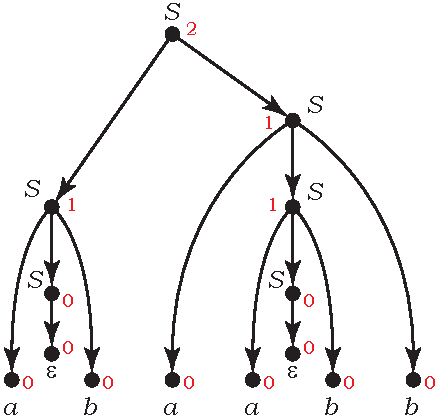
\includegraphics[scale=0.9]{tree_dimension_example}
\caption{A parse tree with marked dimensions of its subtrees.}
\label{f:tree_dimension_example}
\end{figure}

\paragraph{Tree dimension.} 
For each node $v$ in a parse tree $t$,
its \emph{dimension} $\dim v$ is an integer
representing the amount of branching in its subtree.
It is defined inductively: %on the structure of subtrees.
a leaf $v$ has dimension $0$.
%\begin{itemize}
%\item if $v$ is a leaf, then $dim(v)$ = 0
For an internal node $v$, if one of its children $v_1, v_2, \ldots, v_k$, with $k \geqslant 1$,
has a greater dimension than all the others,
then $v$ has the same dimension,
and if there are multiple children of maximum dimension,
then the dimension of $v$ is greater by one.
\begin{equation*}
	\dim v
		=
	\begin{cases}
	\max_{i \in \{1, \ldots, k\}} \dim v_i
		&\text{if there is a unique maximum} \\
	\max_{i \in \{1, \ldots, k\}} \dim v_i +1
		&\text{otherwise}
	\end{cases}
\end{equation*}
The dimension of a parse tree $t$, denoted by $\dim t$, is the dimension of its root.
%It is observable from the definition that the dimension of a tree $t$
%This is the height of the largest perfect binary tree,
%obtained from $t$ by contracting edges and identifying vertices.
An example of a parse tree with marked dimensions of its nodes
is given in Figure~\ref{f:tree_dimension_example},
it uses a grammar for the Dyck language ($S \to SS \ | \ aSb \ | \ \epsilon$).

%A tree of dimension $dim(t) = 2$ is illustrated in Figure~\ref{oscbtree}.

\begin{definition}[Grammars of bounded tree dimension]
Let $d \geqslant 1$.
A grammar $G$ is said to be of tree dimension bounded by $d$,
if every parse tree $t$ of $G$ has $\dim t \leqslant d$,
The least such constant $d$ is called the dimension of $G$,
denoted by $\dim G=d$.
\end{definition}

%\ao{Never used!}
%Languages defined by such grammars shall be called \emph{languages of $d$-bounded tree dimension}.






\section{Upper bound on the rational index}\label{section_upper_bound} % of languages of bounded tree dimension}

The first result of this paper
is that, if the dimension of trees in a grammar is bounded by a constant $d$,
then the rational index of its language is bounded by $O(n^{2d})$,
where the constant factor depends upon the grammar.

\begin{theorem}\label{rational_index_upper_bound_theorem}
Let $G$ be a grammar of tree dimension bounded by $d$,
and let $\mathcal{A}$ be an NFA with $n$ states,
with non-empty intersection $L(G) \cap L(\mathcal{A})$.
Then the length of the shortest string in $L(G) \cap L(\mathcal{A})$ is in $O(n^{2d})$.
\end{theorem}

The main component of the proof
is the following lemma by Chytil and Monien~\cite{ChytilMonien},
which they used in their study of unambiguous grammars of finite index.

\begin{lemma}[Chytil and Monien~{\cite[Lem.~7]{ChytilMonien}}]\label{lem_caterpillars}
%Let $G$ be an arbitrary context-free grammar,
%$r$ the number of its nonterminals
%and $\ell$ the maximal length of the right-hand side of its rules.
%Then for every derivation $d$-caterpillar tree $t$
%describing a derivation $X\stackrel {*}{\Rightarrow } w$,
%where $X$ is a nonterminal and $w$ is a terminal string,
%there exist a $d$-caterpillar derivation tree $t'$
%describing a derivation $X\stackrel {*}{\Rightarrow } w'$ of some terminal string $w'$
%such that
%$$|w'|\leqslant (r(\ell-1) + 1)^{d}.$$
%
Let $G=(\Sigma, N, R, S)$ be a grammar,
let $m$ %=\max_{A \to \alpha \in R} |\alpha|$
be the maximal length of the right-hand side of its rules,
and assume that there exists a parse tree of some dimension $d \geqslant 1$ in this grammar.
Then the grammar defines some string
%hortest string defined by the grammar
of length at most $(|N|(m-1) + 1)^d$.
\end{lemma}
\begin{proof}
A proof is included for completeness;
later in Section~\ref{section_multi_upper_bound}
it will be generalized for multi-component grammars.

For each nonterminal $A$ that has at least one parse tree of some dimension $d$,
it is proved that $A$ defines some string of length at most $(|N|(m-1) + 1)^d$.
The proof proceeds by induction on $d$.

Base case: $d=0$.
If $A$ defines a tree of dimension 0,
then the yield of this tree is a string of length 0 or 1.

Induction step: $d -1 \to d$.
Let $w$ be the shortest string defined by $A$ with a parse tree of dimension at most $d$,
and among all such parse trees, let $t$ be the one with the fewest nodes.
Consider the path in $t$ that proceeds from its root
and passes through nodes of dimension $d$.
If all children of the root have dimension $d-1$,
then this path consists of a single node;
otherwise, one of the children of the root has dimension $d$,
and other children have dimension less than $d$,
and the path continues to the child of dimension $d$, etc.
Such a path is illustrated in Figure~\ref{f:chytil_monien_main_path}.

Let $A_1, \ldots, A_h$ be the nonterminals in the labels of nodes on this path,
with $A_1=A$.
%Then the one with dimension $d$ may also have one child of dimension $d$, etc.
No nonterminal symbol is repeated twice in this sequence,
because if $A_i=A_j$ for some $i<j$,
then the segment of this path from $A_{i+1}$ to $A_j$
could be contracted,
and the resulting parse tree would either define a string shorter than $w$,
or would be a smaller tree of $w$,
while still having dimension at most $d$.
Therefore, $h \leqslant |N|$.

\begin{figure}[t]
\centering
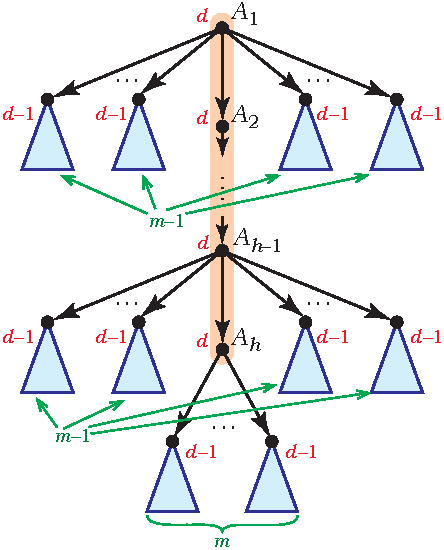
\includegraphics[scale=0.9]{chytil_monien_main_path}
\caption{The path passing through nodes of dimension $d$ in the proof of the Chytil--Monien lemma.}
\label{f:chytil_monien_main_path}
\end{figure}

For each node on this path except the last one,
at most $m-1$ subtrees
may spawn off to the left and to the right,
and each of them has dimension less than $d$.
The last node on this path has at most $m$ children, all of dimension less than $d$.
Overall, there are at most $(m-1) \cdot (h-1) + m \leqslant (m-1)(|N|-1)+m = |N|(m-1) + 1$ subtrees,
each of dimension at most $d-1$.
Each of these subtrees, with some root $X \in \Sigma \cup N$,
defines one of the shortest strings in $L_G(X)$,
and therefore, by the induction hypothesis,
the substring in each subtree is of length at most $(|N|(m-1) + 1)^{d-1}$.
Since $w$ is the concatenation of these substrings,
its length is at most $(|N|(m-1) + 1)^{d-1} \cdot (|N|(m-1) + 1) = (|N|(m-1) + 1)^d$,
as claimed.
\qed
\end{proof}

\begin{proof}[of Theorem~\ref{rational_index_upper_bound_theorem}]
Let $N$ be the set of nonterminal symbols in $G$.
A grammar $G'$ for the language $L(G) \cap L(\mathcal{A})$
is obtained from $G$ and $\mathcal{A}$
by the classical construction by Bar-Hillel et al.~\cite{BarHillel},
which produces $|N| \cdot n^2 + 1$ nonterminal symbols:
these are all triples of the form $(A, p, q)$, where $A \in N$
and $p,q$ are two states of the automaton,
as well as a new start symbol.
Furthermore, each parse tree in the grammar $G'$
has the same structure as some parse tree in $G$,
and differs only in the labelling of internal nodes;
in particular, it has the same dimension.

Since $G'$ defines at least one string,
the parse tree of that string has the same dimension as some parse tree in $G$,
and its dimension is therefore at most $d$.
Let $m$ be the maximum length of the right-hand sides of rules in $G'$.
Then, by Lemma~\ref{lem_caterpillars},
the length of the shortest string defined by $G'$
is at most 
$((|N| \cdot n^2 + 1) (m-1) + 1)^d = |N| \cdot (m-1) \cdot n^{2d} + o(n^{2d}) = O(n^{2d})$.
\qed
\end{proof}







\section{Lower bound on the rational index}\label{section_lower_bound} % of languages of bounded tree dimension}

The upper bound $O(n^{2d})$ on the rational index of a language
defined by a grammar with tree dimension bounded by $d$
has a matching lower bound $\Omega(n^{2d})$.
It is first established for a convenient infinite set of values of $n$,
to be extended to arbitrary $n$ in the following.

\begin{lemma}\label{rational_index_lower_bound_lemma}
For every $d \geqslant 1$,
there is a grammar $G$ of tree dimension bounded by $d$,
such that for every $n \geqslant 2^{d+1}$ divisible by $2^d$
there is an $n$-state partial DFA $\mathcal{B}$,
such that the shortest string $w$ in $L(G) \cap L(\mathcal{B})$
is of length at least $\frac{1}{2^{d^2 + 3d - 3}} n^{2d}$.
\end{lemma}
\begin{proof}
The proof is carried out by induction on $d$.
A grammar is constructed for each $d$,
and then, for every $n$ divisible by $2^d$,
an $n$-state DFA with the stated property is defined.
Each constructed automaton shall have a unique initial state,
which is also the unique accepting state.

\textbf{Basis:} $dim(G) = 1$.
The family of languages having dimension $d = 1$
coincides with the family of linear languages.
Let $G$ be a linear grammar with the rules $S \to aSb \ | \ ab$,
which defines the language $L(G) = \set{a^i b^i}{i \geqslant 1}$. 

For every $n \geqslant 4$ divisible by $2^d=2$,
let $\ell = \frac{n}{2}$ and $m=\frac{n}{2} + 1$.
Then $\ell$ and $m$ are coprime integers.
Define a DFA $\mathcal{B}$ over the alphabet $\{a, b\}$,
which consists of two cycles
sharing one node, $q_0$,
which is both the initial and the unique accepting state.
The cycle of length $\ell$ has all transitions by $a$, and the other by $b$,
as shown in Figure~\ref{worstd_1}.
The automaton has $\ell+m-1=n$ states.

Every string in $L(G) \cap L(\mathcal{B})$
is of the form $a^i b^i$, with $i \geqslant 1$.
For the automaton to accept it,
$i$ must be divisible both by $\ell$ and by $m$.
Since the cycle lengths are relatively prime,
the shortest string $w$ with this property has $i=\ell m$,
and is accordingly of length $2\ell m$.
Its growth with $n$ is estimated as follows.
\begin{equation*}
	|w|
		=
	2\ell m
		=
	2 \frac{n}{2} \cdot \Big(\frac{n}{2} + 1\Big)
		=
	\frac{1}{2} n^2 + n
\end{equation*}
This example is well-known to the community~\cite{HellingsCFPQ,Yannakakis}. 

\begin{figure}[t]
\centering
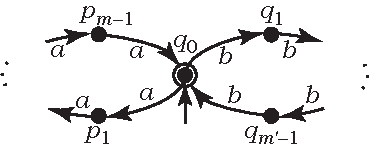
\includegraphics[scale=0.9]{rational_index_A1.pdf}
\caption{DFA $\mathcal{B}$ defined in Lemma~\ref{rational_index_lower_bound_lemma} for $d=1$.}
\label{worstd_1}
\end{figure}

\textbf{Induction step:} $dim(G) = d$.
By the induction hypothesis,
there is a grammar $\widehat{G} = (\widehat{\Sigma}, \widehat{N}, \widehat{R}, \widehat{S})$
of bounded tree dimension $dim(\widehat{G}) = d-1$,
which satisfies the statement of the lemma.
The new grammar $G = (\Sigma, N, R, S)$ of tree dimension at most $d$
is defined over the alphabet 
$\Sigma = \widehat{\Sigma} \cup \{a, b, c\}$,
where $a, b, c \not\in \widehat{\Sigma}$ are new symbols.
It uses nonterminal symbols
$N = \widehat{N} \cup \{S, A\}$,
adding two new nonterminals $A, S \not\in \widehat{N}$ to those in $\widehat{G}$,
where $S$ is the new initial symbol.
Its set of rules includes all rules from $\widehat{G}$
and the following new rules.
\begin{align*}
	S &\to A S c \ | \ A c \\
	A &\to a A b \ | \ a \widehat{S} b
\end{align*}
Here the nonterminal symbol $A$ defines all substrings of the form $a^i u b^i$,
with $i \geqslant 1$ and $u \in L(\widehat{G})$,
and hence the grammar defines the following language.
\begin{equation*}
	L(G)=\set{a^{i_1} w_1 b^{i_1} \ldots a^{i_t} w_t b^{i_t} c^t}{t \geqslant 1, \:
		i_1, \ldots, i_t \geqslant 1, \:
		w_1, \ldots, w_t \in L(\widehat{G})}
\end{equation*}

\begin{figure}[t]
\centering
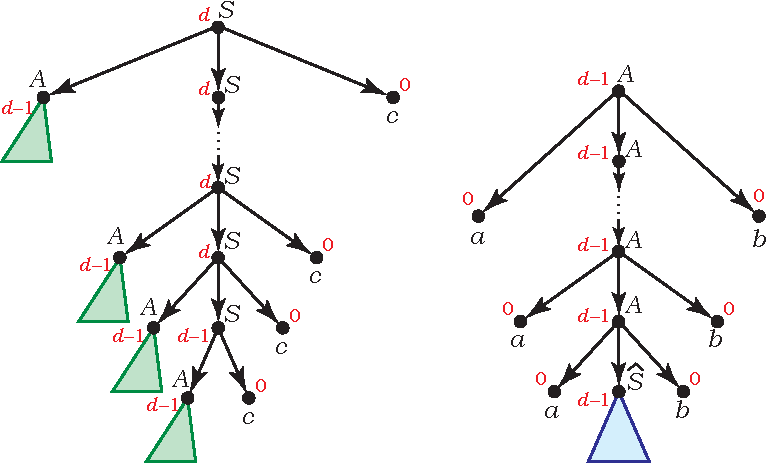
\includegraphics[scale=0.9]{rational_index_parse_tree_S_A.pdf}
\caption{Parse trees for $S$ and for $A$, annotated with dimensions of their nodes.}
\label{dimsubtree}
\end{figure}

To see that trees in the new grammar have dimension at most $d$,
first consider the dimension of any parse tree $t$ with the root labeled by the nonterminal $A$,
which is of the form shown in Figure~\ref{dimsubtree}(right).
The dimension of the $\widehat{S}$-subtree at the bottom
is at most $d-1$ by the properties of $\widehat{G}$.
This dimension is inherited by all $A$-nodes in the tree,
because their remaining children are leaves.
%Multiple applications of the rule $A \to a A b$
%do not increase the dimension of the parse tree,
%because the dimensions of nodes labeled with $a$, $b$ are equal to $0$.

Now consider the dimension of a complete parse tree $t$ with the start symbol $S$ in the root,
as in Figure~\ref{dimsubtree}(left).
All $A$-subtrees in this tree have dimension at most $d-1$.
Then the bottom $S$-subtree, which uses the rule $S \to Ac$,
also has dimension at most $d-1$.
Every $S$-subtree higher up in the tree uses a rule $S \to ASc$,
and its dimension is at most $d$,
because getting a higher dimension would require two subtrees of dimension $d$,
which is never the case.
%As there is no unique maximum, $dim(t) = \max_{i} (v_i) + 1 = d - 1 + 1 = d$.
%Notice that only one application of the rule $S \to A S c$ increases the dimension of $t$,
%whereas further applications do not make any effect on the dimension of parse tree.

Now, for every $n \geqslant 2^{d+1}$ divisible by $2^d$,
the goal is to construct an $n$-state DFA over the alphabet $\Sigma$,
so that the shortest string $w$ in $L(G) \cap L(\mathcal{B})$
is of length at least $\frac{1}{2^{d^2 + 3d - 3}} n^{2d}$.
Since the number $\frac{n}{2}$ is at least $2^d$ and is divisible by $2^{d-1}$,
the induction hypothesis for the grammar $\widehat{G}$
asserts that there is a DFA
$\widehat{\mathcal{B}} = (\widehat{Q}, \widehat{\Sigma}, \widehat{\delta}, \widehat{q}_0, \{\widehat{q}_0\})$,
with $\frac{n}{2}$ states,
with the shortest string $\widehat{w}$ in $L(\widehat{G}) \cap L(\widehat{\mathcal{B}})$
of length at least $\frac{1}{2^{(d-1)^2 + 3(d-1) - 3}} (\frac{n}{2})^{2(d-1)}$.

The desired $n$-state DFA $\mathcal{B} = (\Sigma, Q, q_0, \delta, \{q_0\})$
is constructed as follows.
Let $\ell = \frac{n}{4}$ and $m=\frac{n}{4} + 1$, these are two coprime integers.
The set of states of $\mathcal{B}$
contains all $\frac{n}{2}$ states from $\widehat{Q}$,
in which $\mathcal{B}$ operates as $\widehat{\mathcal{B}}$,
and $m+\ell-1=\frac{n}{2}$ new states forming
a cycle of length $\ell$ and a chain of length $m$,
which share a common state $q_0$.
\begin{equation*}
	Q = \widehat{Q} \cup \{p_1, \ldots, p_{\ell-1}, q_0, \ldots, q_{m-1}\}
\end{equation*}
The new initial state $q_0$ has a transition by $a$
leading to the initial state of $\widehat{\mathcal{B}}$,
from where one can return to $q_1$ by $b$.
\begin{align*}
	\delta(q_0, a) &= \widehat{q}_0
		\\
	\delta(\widehat{q}_0, b) &= q_1
\intertext{%
There is a chain of transitions by $a$ from $q_{m-1}$ to $q_0$,
and another chain $b$ in the opposite direction, from $q_1$ to $q_{m-1}$ and back to $q_0$.
}
	\delta(q_i, a) &= q_{i-1},
		&& \text{with } 1 \leqslant i \leqslant m-1
		\\
	\delta(q_i, b) &= q_{i+1 \bmod m},
		&& \text{with } 1 \leqslant i \leqslant m-1
\intertext{%
There is a cycle by $c$ in the states $q_0, p_1, \ldots, p_{\ell-1}$;
for uniformity, denote $p_0=q_0$.
}
	\delta(p_i, c) &= p_{i+1 \bmod \ell},
		&& \text{with } 0 \leqslant i \leqslant \ell-1
\end{align*}
The general form of $\mathcal{B}$ is shown in Figure~\ref{dimautomata:generalized}.

\begin{figure}[t]
	\centering
	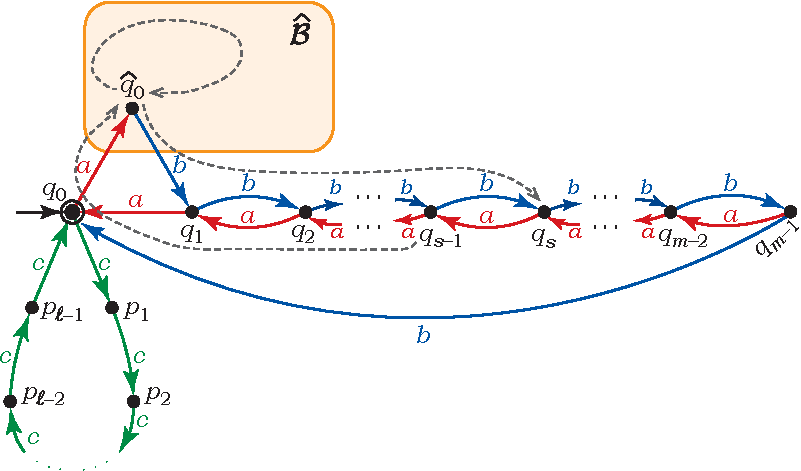
\includegraphics[scale=0.9]{rational_index_Ad}
	\caption{DFA $\mathcal{B}$ defined in Lemma~\ref{rational_index_lower_bound_lemma} for $d$,
		which incorporates DFA $\widehat{\mathcal{B}}$ for $d-1$.
		A computation on a block $a^{i_s} w_s b^{i_s}$
		that starts in $q_{s-1}$ and ends in $q_s$ is illustrated.}
	\label{dimautomata:generalized}
\end{figure}

Let $w$ be any string in $L(G) \cap L(\mathcal{B})$.
Since $w$ is defined by $G$,
it is of the form 
$w = a^{i_1} w_1 b^{i_1} \ldots a^{i_t} w_t b^{i_t} c^t$,
for some $t \geqslant 1$,
$i_1, \ldots, i_t \geqslant 1$
and $w_1, \ldots, w_t \in L(\widehat{G})$.
At the same time, $w$ must be accepted by $\mathcal{B}$,
and the automaton's behaviour on $w$ is explained in the following claim.

\begin{claim}
After reading each prefix $a^{i_1} w_1 b^{i_1} \cdots a^{i_s} w_s b^{i_s}$ of $w$,
with $s \in \{0, \ldots, t\}$,
the automaton comes to the state $q_{s \bmod m}$.
%and $i_s$ must be equal to $(s-1 \bmod m)+1$.
\end{claim}
\begin{proof}
The claim is proved by an induction on $s$.
For the base case, $s=0$, it holds true,
because the initial state is $q_0$.

For the induction step,
assume that the automaton is in the state $q_{(s-1) \bmod m}$
after reading $a^{i_1} w_1 b^{i_1} \cdots a^{i_{s-1}} w_{s-1} b^{i_{s-1}}$
and it reads the next block $a^{i_s} w_s b^{i_s}$;
it is claimed that it must finish reading this block
in the state $q_{s \bmod m}$.
For the automaton to read any symbols of $w_s$,
it must come to the state $\widehat{q}_0$,
which is possible only if $i_s = ((s-1) \bmod m) + 1$;
hence, $i_s$ is at most $m$.
Similarly, for the automaton to continue reading $b^{i_s}$
after processing $w_s$,
it must finish reading $w_s$ in the state $\widehat{q}_0$.
Then, by reading the string $b^{i_s}$,
it gets to the state $q_{i_s \bmod m}$.
If $i_s < m$, then $(s-1) \bmod m < m-1$
and $i_s = s \bmod m$, and the state reached is $q_{s \bmod m}$, as claimed
(this is the case illustrated in Figure~\ref{dimautomata:generalized}).
If $i_s = m$, then $(s-1) \bmod m = m-1$,
and the automaton reaches $q_0$; since $s \bmod m = 0$, this is the claimed state.
The proof of the claim is complete.
\qed
\end{proof}

Resuming the proof of the lemma,
it is now known that the automaton starts reading the suffix $c^t$ of $w$
in the state $q_{t \mod m}$.
Unless this is the state $q_0$,
symbols $c$ cannot be read.
Therefore, $t$ must be divisible by $m$.
At the same time, in order to finish reading $c^t$ in the accepting state,
$t$ must also be divisible by $\ell$.
Furthermore, in such a string,
each substring $w_i$ must be accepted by $\widehat{\mathcal{B}}$,
because $\mathcal{B}$ starts and finishes reading it in the state $\widehat{q}_0$,
and therefore lies in $L(\widehat{G}) \cap L(\widehat{\mathcal{B}})$,
and its length is at least $|\widehat{w}|$,
where $\widehat{w}$ is the shortest string in $L(\widehat{G}) \cap L(\widehat{\mathcal{B}})$.

Then, the shortest string $w$ with these properties
must have $t=\ell m$,
because $\ell$ and $m$ are co-prime,
and must have each $w_i$ of length exactly $|\widehat{w}|$.
This gives the following lower bound on the length of $w$.
\begin{multline*}
	|w|
		>
	\ell m |\widehat{w}|
		\geqslant
	\frac{n}{4} \cdot \frac{n}{4} \cdot 
	\frac{1}{2^{(d-1)^2 + 3(d-1) - 3}} \Big(\frac{n}{2}\Big)^{2(d-1)}
		= \\ = %d^2 -2d + 1 + 3d -3 - 3 = d^2 + d - 5
	\frac{n^2}{16} \cdot 
	\frac{1}{2^{d^2 + d - 5}} \cdot \frac{n^{2d-2}}{2^{2d-2}}
		= %d^2 + d - 5 + 4 + 2d - 2 = n^2 + 3d -3
	\frac{1}{2^{d^2 + 3d -3}} n^{2d}
\end{multline*}
The estimation uses that $\ell$ and $m$ are at least $\frac{n}{4}$,
and invokes the induction hypothesis to get a lower bound on $|\widehat{w}|$.
\qed
\end{proof}

\begin{comment}
Recall that NFA $\widehat{\mathcal{B}}$ has $\frac{n}{2}$ states, $m = \frac{n}{4} +1$ and $\ell = \frac{n}{4}$.

For $d=1$, $|w| = |w_1| = \frac{1}{2} n^2 + n\geqslant \frac{1}{2} n^2$.

For $d=2$, $|w| = |w_2| \geqslant m \ell |w^{(\frac{n}{2})}_1| \geqslant \frac{n}{4} \frac{n}{4} \frac{1}{2} { (\frac{n}{2}) }^2 =  \frac{n^2}{16} \frac{1}{2} \frac{n^2}{4} = \frac{n^4}{128}$.

For $d=3$, $|w| = |w_3| \geqslant m \ell |w^{(\frac{n}{2})}_2| \geqslant \frac{1}{16} n^2 ( \frac{1}{16} {(\frac{n}{2}) }^2 |w^{(\frac{n}{4})}_1| )$.

Thus, for any $d$:
\begin{multline*}
	|w| \geqslant  \left(\frac{1}{16}\right)^{d-1} \cdot n^{2(d-1)}  \cdot \left(\frac{1}{2}\right)^2 \cdot \left(\frac{1}{4}\right)^2 \cdot \ldots \cdot \left(\frac{1}{2^{d-2}}\right)^2 \cdot \left|w^{\left(\frac{n}{2^{d-1}}\right)}_1\right| 
	\geqslant \\ \geqslant
	 \left(\frac{1}{16}\right)^{d-1} \cdot n^{2(d-1)} \cdot \left(\frac{1}{2\cdot 4 \cdot \ldots \cdot 2^{d-2}} \right)^{2} \cdot \frac{1}{2} \cdot \left(\frac{1}{2^{d-1}}\right)^2 n^{2} 
	= \\ =
	 \frac{1}{2} \cdot \left(\frac{1}{16}\right)^{d-1} \cdot \left(\frac{1}{2\cdot 4 \cdot \ldots \cdot 2^{d-1}} \right)^{2} \cdot n^{2d} 
	= \\ =
     \frac{1}{2^{1 + 4d - 4 + 2(1 + 2 + \ldots d-1)}} \cdot n^{2d} = \frac{n^{2d}}{2^{d^2 + 3d - 3}}
\end{multline*}
\end{comment}

\begin{theorem}\label{lower_bound_theorem}
For every $d \geqslant 1$,
there is a grammar $G$ of bounded tree dimension $d$,
such that for every $n \geqslant 2^{d+1}$
there is an $n$-state partial DFA $\mathcal{B}$,
such that the shortest string $w$ in $L(G) \cap L(\mathcal{B})$
is of length greater than $\frac{1}{2^{d^2 + d - 3} 3^{2d}} n^{2d}$.
\end{theorem}
\begin{proof}
Let $G$ be the grammar given for $d$ by Lemma~\ref{rational_index_lower_bound_lemma}.
Let $2^d r \leqslant n < 2^d (r+1)$, for some integer $r$.
Then $r \geqslant 2$ (for otherwise $n < 2^{d+1}$),
and $2^d r \geqslant 2^{d+1}$.

Since $2^d r$ is divisible by $2^d$,
by Lemma~\ref{rational_index_lower_bound_lemma},
there is a DFA $\mathcal{B}$ with $2^d r \leqslant n$ states,
such that the length of the shortest string $w$ in $L(G) \cap L(\mathcal{B})$
is at least $\frac{1}{2^{d^2 + 3d - 3}} (2^d r)^{2d}$.
This is the desired $n$-state DFA.

%(r/(r+1) >= 2/3, 3r/2(r+1) >= 1)
%n < 2^d (r+1) <= 2^d (r+1) 3r/2(r+1) = 3/2 2^d r
%2/3n < 2^d r

The inequality $n < 2^d (r+1)$ implies that $n < 2^d \frac{3r}{2}$,
because $r+1$ is at most $\frac{3r}{2}$ for $r \geqslant 2$.
Then $2^d r > \frac{2}{3}n$,
and the lower bound on the length of $w$ is expressed as a function of $n$
as follows.
\begin{equation*}
	|w|
		\geqslant
	\frac{1}{2^{d^2 + 3d - 3}} (2^d r)^{2d}
		>
	\frac{1}{2^{d^2 + 3d - 3}} \big(\frac{2}{3} n\big)^{2d}
		=
	\frac{1}{2^{d^2 + d - 3} 3^{2d}} n^{2d}
\end{equation*}
\qed
\end{proof}

For finite automata with fewer than $2^{d+1}$ states,
no lower bounds are given,
as the construction in the proof relies on having sufficiently long cycles in the automata.

Overall,
the rational index of grammars with tree dimension bounded by $d$
is $\Theta(n^{2d})$ in the worst case.


\begin{comment}
Let $m = 2^dr = n - q$.
Then
\begin{align*}
	n > m > 2^{d+1} 
\\
   \frac{n}{2} > 2^d > q
\\
  (n-q)^{2d} \geqslant \left( \frac{n}{2}\right)^{2d}
\end{align*}
Consider an NFA $\widehat{\mathcal{B}}$ with $m = n - q = 2^d r$ states. By Lemma~\ref{rational_index_lower_bound_lemma} the shortest string $\widehat{w}$ in $L(G) \cap L(\mathcal{B})$
is of length at least $\frac{m^{2d}}{2^{d^2 + 3d - 3}} = \frac{(n-q)^{2d}}{2^{d^2 + 3d - 3}}$.

But $(n-q)^{2d} \geqslant \left( \frac{n}{2}\right)^{2d}$ and, therefore, $\frac{(n-q)^{2d}}{2^{d^2 + 3d - 3}} \geqslant\frac{(n)^{2d}}{2^{2d} \cdot 2^{d^2 + 3d - 3}} = \frac{(n)^{2d}}{2^{d^2 + 5d - 3}}$. \qed
\end{comment}







\section{Tree dimension in multi-component grammars}\label{section_multi}

Multi-component grammars define the structure of a sentence $w$
by splitting it into constituents that are finite $k$-tuples of disjoint substrings of $w$,
for $k$ bounded by a constant.
In other words, these are substrings with $k-1$ gaps,
and these constituents can be joined to each other
by concatenating their components from any sides.
In all other respects, these grammars are the same as ordinary (context-free) grammars.

\begin{definition}[Vijay-Shankar, Weir, Joshi~\cite{VijayshankarWeirJoshi};
	Seki, Matsumura, Fujii, Kasami~\cite{SekiMatsumuraFujiiKasami}]
\label{multi_definition}
A multi-component grammar is a quintuple
$G=(\Sigma, N, \ranksymb, R, S)$,
where
\begin{itemize}
\item
	$\Sigma$ is the alphabet of the language being described;
\item
	$N$ is the set of nonterminal symbols;
\item
	$\ranksymb \colon N \to \mathbb{N}$
	is a function that defines
	the number of components in each nonterminal symbol,
	so that if $\rank{A}=k$,
	then $A$ describes $k$-tuples of substrings;
\item
	$R$ is a set of grammar rules,
	each of the form
	\begin{equation}\tag{*}\label{multi_component_rule}
		A(\alpha_1, \ldots, \alpha_{\rank{A}})
			\leftarrow
		B_1(x_{1,1}, \ldots, x_{1, \rank{B_1}}),
		\ldots,
		B_\ell(x_{\ell,1}, \ldots, x_{\ell, \rank{B_\ell}}),
		%
		%A
		%	\to
		%f(B_1, \ldots, B_m),
	\end{equation}
	where $\ell \geqslant 0$,
	the variables $x_{i,j}$ are pairwise distinct,
	$\alpha_1, \ldots, \alpha_{\rank A}$
	are strings over symbols from $\Sigma$ and variables $x_{i,j}$,
	and each variable $x_{i,j}$
	occurs in $\alpha_1 \ldots \alpha_{\rank A}$ exactly once;
\item
	a nonterminal symbol $S \in N$ of dimension 1
	is the ``initial symbol'',
	that is, the category of all well-formed sentences defined by the grammar.
\end{itemize}
A grammar is seen as a logical system
for proving elementary propositions of the form
$A(w_1, \ldots, w_k)$,
with $k=\rank{A}$ and $w_1, \ldots, w_k \in \Sigma^*$,
meaning that the given $k$-tuple of strings has the property $A$.
A proof proceeds using the rules in $R$,
with each rule (\ref{multi_component_rule})
treated as a schema for derivation rules,
for any strings substituted for all variables $x_{i,j}$.
\begin{equation*}
	\infer{A(\alpha_1, \ldots, \alpha_{\rank{A}})}{
		B_1(x_{1,1}, \ldots, x_{1, \rank{B_1}})
		& \ldots &
		B_\ell(x_{\ell,1}, \ldots, x_{\ell, \rank{B_\ell}})
	}
\end{equation*}
The language generated by the grammar,
denoted by $L(G)$,
is the set of all such strings $w$
that the proposition $S(w)$
can be derived in one or more such steps.

The rank of a grammar, $\rank{G}$, is the largest rank of a nonterminal symbol.
A multi-component grammar of rank $k$
shall be called a $k$-component grammar.
\end{definition}

Whenever a string $w$ is generated by $G$,
the derivation of a proposition $S(w)$
forms a \emph{parse tree}.
Each node in the tree is labelled with a proposition $A(w_1, \ldots, w_k)$,
where $k=\rank{A}$ and $w_1, \ldots, w_k$ are substrings of $w$.
Every node has a corresponding rule (\ref{multi_component_rule}),
by which the proposition is derived,
and the direct successors of this node
are labelled with $B_1(x_{1,1}, \ldots, x_{1, \rank{B_1}})$,
	\ldots,
$B_\ell(x_{\ell,1}, \ldots, x_{\ell, \rank{B_\ell}})$,
as in the definition of a derivation step.

\begin{comment}
The definition of rules in a multi-component grammar
may be relaxed
to have each variable $x_{i,j}$
occur in $\alpha_1 \ldots \alpha_{\rank A}$ \emph{at most} once.
However, it is known that every such grammar can be transformed
to eliminate unused variables,
to match Definition~\ref{multi_definition}.
\end{comment}

\begin{comment}
The ability of multi-component grammars to permute the components arbitrarily
is actually inessential:
one can assume that each rule is \emph{non-permuting},
that is, preserves the order of the components in the resulting string.

\begin{proposition}\label{multi_to_nonpermuting_proposition}
Each $k$-component grammar
is equivalent to a $k$-component \emph{non-permuting} grammar,
in which, for every rule~\eqref{multi_component_rule}
and for every $i$,
the variables $x_{i,1}, \ldots, x_{i,\dim{B_i}}$ occur inside $\alpha_1 \ldots \alpha_{\dim{A}}$
in the order listed.
\end{proposition}

In a non-permuting grammar, whenever a proposition $A(w_1, \ldots, w_k)$
is used in a derivation of $S(w)$,
the substrings $w_1, \ldots, w_k$ occur in $w$ exactly in this order,
that is, $w=x_0 w_1 x_1 w_2 \ldots x_{k-1} w_k x_k$ for some $x_0, \ldots, x_k \in \Sigma^*$.

\paragraph{Well-nested multi-component grammars}
are a special case of multi-component grammars,
in which, whenever multiple constituents are joined in a single rule,
their components cannot be intertwined,
unless one's components are completely embedded
within another's components.
Thus, patterns such as
$A(x_1y_1, x_2y_2) \leftarrow B(x_1, x_2) C(y_1, y_2)$
are prohibited.

\begin{definition}
A non-permuting multi-component grammar is called well-nested,
if, in every rule~\eqref{multi_component_rule},
%satisfies the following condition:
%		A(\alpha_1, \ldots, \alpha_{\rank{A}})
%			\leftarrow
%		B_1(x_{1,1}, \ldots, x_{1, \rank{B_1}}),
%		\ldots,
%		B_\ell(x_{\ell,1}, \ldots, x_{\ell, \rank{B_\ell}}),
%\begin{enumerate}
%\item
%	(non-permuting condition)
%	For every $i$,
%	the variables $x_{i,1}, \ldots, x_{i,\dim{B_i}}$ occur inside $\alpha_1 \ldots \alpha_{\dim{A}}$
%	in this particular order.
%\item
	for all $i, i'$, with $i \neq i'$,
	the concatenation $\alpha_1 \ldots \alpha_{\dim{A}}$
	satisfies one of the following patterns:
	\begin{itemize}
	\item
		$\ldots x_{i', d_{i'}} \ldots x_{i, 1} \ldots$,
		that is, all components of $B'_i$ come before the first component of $B_{i}$;
	\item
		$\ldots x_{i,r} \ldots x_{i',1} \ldots x_{i',d_{i'}} \ldots x_{i,r+1} \ldots$,
		that is, all components of $B'_i$
		are listed between two consecutive components of $B_{i}$;
	\item
		$\ldots x_{i, d_i} \ldots x_{i', 1} \ldots$,
		that is, all components of $B'_i$ come after the last component of $B_{i}$.
	\end{itemize}
%\end{enumerate}
\end{definition}

From the linguistic point of view,
this means that the span of a constituent
cannot be intertwined with another constituent's components,
unless one is enclosed within the other.
\end{comment}
\begin{example}\label{exam-well-nested}
The language $L = \set{a^m b^n c^m d^n}{m, n \in \mathbb{N}}$
is defined by the following %well-nested 
$2$-component grammar.
\begin{align*}
	S(xy) &\leftarrow A(x, y) \\
	A(x, byd) &\leftarrow A(x, y) \\
	A(x, y) &\leftarrow B(x, y) \\
	B(\epsilon, \epsilon) &\leftarrow \\
	B(ax, cy) &\leftarrow B(x, y)
\end{align*}
Here $B$ defines all pairs $(a^m, c^m)$, with $m \geqslant 0$,
and $A$ defines all pairs $(a^m, b^n c^m d^n)$, with $m,n \geqslant 0$.
Finally $S$ concatenates every such pair to a string in $L$.
\end{example}
\begin{comment}
Well-nested multi-component grammars
are strictly weaker than the general case:
e.g., the language $\set{wcw}{w \in L_0}$, where $L_0 \subseteq \{a,b\}^*$ is the Dyck language,
is defined by a 2-component grammar,
but by no well-nested $k$-component grammar, regardless of $k$~\cite{KanazawaSalvati}.
\end{comment}

\paragraph{Tree dimension.}
The conventional definition of parse trees for multi-component grammars
does not include the terminal symbols in the tree structure,
and this makes it incompatible with ordinary parse trees in terms of tree dimension.
To keep the definitions compatible,
for each node in which a rule of the form (\ref{multi_component_rule}) is applied,
every occurrence of a terminal symbol on the left-hand side of this rule
shall be regarded as an extra leaf attached to this node,
along with proper children labelled with $B_1$, \ldots, $B_\ell$.
Each of these extra leaves has dimension 0.
%and may affect the dimension of their parent,
% if their parent would otherwise have dimension 0.
The dimension of every node is then defined inductively
on the dimensions of its children, as usual.

\begin{definition}[Grammars of bounded tree dimension]
A multi-component grammar $G$ is said to be of tree dimension bounded by $d$
if every parse tree has dimension at most $d$.
The least such constant $d$ is called the dimension of $G$, denoted by $\dim G=d$.
\end{definition}

\begin{comment}
A well-nested multi-component grammar
can be transformed to the following form
resembling the Chomsky normal form.

\begin{proposition}[{\cite[Thm.~1]{Sorokin2013}}]\label{wn_multi_normal_form_proposition}
Each well-nested $k$-component grammar
is equivalent to a well-nested $k$-component grammar,
in which all rules are of the following form.
\begin{align*}
	A(x_1, \ldots, x_{m-1}, x_m y_1, y_2, \ldots, y_n)
	%A(\mathbf{x}\mathbf{y})
	&\gets
	B(x_1, \ldots, x_m), C(y_1, \ldots, y_n)
	%B(\mathbf{x}), C(\mathbf{y}),
%		&& B, C \neq S
		\\
	A(x_1, \ldots, x_i, x_i y_1, y_2, \ldots y_n x_{i+1}, x_{i+2}, \ldots, x_m)
	%(\mathbf{x} \odot_k \mathbf{y})
	&\gets
	B(x_1, \ldots, x_m), C(y_1, \ldots, y_n)
	%B(\mathbf{x}), C(\mathbf{y}),
%		&& B, C \neq S
		\\
	A(a) &\gets \\
	S(\epsilon) &\gets %\\
%	X(\epsilon, \ldots, \epsilon) &\gets
\end{align*}
Rules of the first kind generalize the concatenation.
The operation implemented in the rules of the second kind,
defined for $i \in \{1, \ldots, m-1\}$,
is known as \emph{displacement}.
\end{proposition}

A multi-component grammar of dimension 1
is an \emph{ordinary grammar},
or ``context-free'' in Chomsky's terminology.
A well-nested multi-component grammar of dimension 2
is known in the literature as a ``head grammar''~\cite{Pollard};
these grammars are equivalent in power to tree-adjoining grammars~\cite{JoshiLevyTakahashi}.
\end{comment}







\section{The Chytil--Monien lemma for multi-component grammars}\label{section_multi_upper_bound}

The rational index of every language
defined by a multi-component grammar of a bounded tree dimension
is bounded by a polynomial that depends both on the tree dimension
and on the maximum number of components in the grammar.
This is proved by a generalization of the proof in Section~\ref{section_upper_bound},
from what was essentially the one-component case to the case of up to $k$ components.

The first step is to adapt the Chytil--Monien lemma~\cite[Lem.~7]{ChytilMonien}.

\begin{lemma}\label{lem_caterpillarsmcfg}
Let $G=(\Sigma, N, \ranksymb, R, S)$ be a multi-component grammar of rank $k$,
let $r$ be the maximum number of nonterminal symbols on the right-hand side of a rule,
let $\ell$ be the maximal number of terminal symbols on the left-hand side of a rule,
and assume that there exists a parse tree of dimension $d \geqslant 1$ in this grammar.
Then the grammar defines some string
of length less than $\frac{\ell+r-1}{r-1} (|N|(r-1) + 1)^d$.
\end{lemma}
\begin{proof}
Let $f(d)$ be the length of the shortest string defined by a grammar of dimension $d$.

It is claimed that $f(0) \leqslant 1$
and $f(d) \leqslant \big(|N|(r-1)+1\big) \cdot f(d-1) + |N| \cdot \ell$.

A parse tree has dimension $d=0$
if it is a path formed of nodes of dimension 0.
The last node on the path defines at most one symbol,
for otherwise it would have dimension greater than zero.
Thus, the length of the shortest string $f(0)$ is at most $1$.

Let $d \geqslant 1$.
Recall the proof of Lemma~\ref{lem_caterpillars} and consider the path from the root 
of the parse tree which passes through the nodes of dimension $d$, where 
every node except the last one has one child of dimension $d$ and other children of dimension 
$d-1$.
As in the proof of Lemma~\ref{lem_caterpillars}, the length of the path is bounded by $|N|$
(otherwise there is a shorter string).
At each node on the path (except the last one)
there are at most $r-1$ subtrees of dimension $d-1$.
The last node of the path has at most $r$ children of dimension $d-1$.
The length of the shortest string defined by a subtree of dimension $d-1$ is $f(d-1)$.
Additionally, at each node, at most $\ell$ extra leaves
listed on the left-hand side of a rule are appended;
in total, there are at most $|N|\ell$ such leaves.

Putting all together, the length of the shortest string is bounded as follows. 
\begin{equation*}
	f(d)
		\leqslant
	\big(|N|(r-1)+1\big) \cdot f(d-1) + |N| \cdot \ell
\end{equation*}

Thus, the length of the shortest string is represented by a recurrence relation
of the form $x_0=1$, $x_d=ax_{d-1} + b$,
where $a=|N|(r-1)+1$ and $b=|N| \cdot \ell$. The upper bound on the solution of this
recurrence relation is as follows. 

\begin{multline*}
	x_d
		=
	a^d + b\frac{a^d-1}{a-1}
		\leqslant 
	a^d + b\frac{a^d}{a-1}
		=
	\Big(\frac{b}{a-1} + 1\Big)a^d
		= \\ =
	\Big(\frac{|N| \cdot \ell}{|N| \cdot (r-1)} + 1\Big)
	\big(|N|(r-1)+1\big)^d
		=
	\frac{\ell + r - 1}{r-1}
	\big(|N|(r-1)+1\big)^d
\end{multline*}
\qed
\end{proof}

The above lemma is used to prove an upper bound
similar to the one in Theorem~\ref{rational_index_upper_bound_theorem}.
The bound gets raised into the power of $k$, the maximum number of components in a grammar,
because the construction for the intersection with a regular languages
produces more nonterminal symbols.

\begin{theorem}\label{rational_index_multi_upper_bound_theorem}
Let $G$ be an multi-component grammar of rank $k$ and of tree dimension bounded by $d$,
and let $\mathcal{A}$ be an NFA with $n$ states,
with non-empty intersection $L(G) \cap L(\mathcal{A})$.
Then the length of the shortest string in $L(G) \cap L(\mathcal{A})$ is at most $O(n^{2kd})$.
\end{theorem}
\begin{proof}
Denote the set of nonterminal symbols in $G$ by $N$.
As proved by Seki et al.~\cite[Thm.~3.9]{SekiMatsumuraFujiiKasami},
for a $k$-component grammar $G$ and an NFA $\mathcal{A}$,
the intersection $L(G) \cap L(\mathcal{A})$
is defined by another $k$-component grammar
with at most $|N| \cdot n^{2k} + 1$ nonterminal symbols.
Their construction generalizes that by Bar-Hillel et al.~\cite{BarHillel},
and produces nonterminal symbols of the form
$(A,p_1, q_1, \ldots, p_{\rank A}, q_{\rank A})$,
where $A \in N$,
$\rank A$ is a rank of the nonterminal $A$, 
and $p_i,q_i$ are states of the automaton,
which it enters before and after reading the corresponding substrings.
The transformation preserves the structure of the parse trees:
each tree in $G'$ has the corresponding tree in $G$
that differs only in the labels of its nodes,
and has the same dimension.

Since the intersection is non-empty, $G'$ defines at least one parse tree,
which has the same dimension as some parse tree in $G$,
that is, at most $d$.
Then, by Lemma~\ref{lem_caterpillarsmcfg},
the shortest string defined by $G'$
is of length at most
$\frac{\ell+r-1}{r-1} ((|N| \cdot n^{2k} + 1)(r-1) + 1)^d$,
where $\ell$ and $r$ are constants depending on $G'$.
This number is estimated as follows.
\begin{multline*}
	\frac{\ell+r-1}{r-1} \big((|N| \cdot n^{2k} + 1)(r-1) + 1\big)^d
		=
	|N| \cdot (\ell+r-1) \cdot n^{2kd} + o(n^{2kd})
		=
	O(n^{2kd})
\end{multline*}
\qed
\end{proof}








\section{A lower bound for multi-component grammars}\label{section_multi_lower_bound}

This section establishes
a lower bound on the rational index of multi-component grammars
that asymptotically matches the bound in Theorem~\ref{rational_index_multi_upper_bound_theorem}.
The main part of the argument is the following lemma
that generalizes Lemma~\ref{rational_index_lower_bound_lemma} to the multi-component case.

\begin{lemma}\label{rational_index_multi_lower_bound_lemma}
For every $d \geqslant 1$, $k \geqslant 2$,
there is a $k$-component grammar $G$ of bounded tree dimension $d$,
such that for every $n \geqslant 8 \cdot 2^d k^2 \ln 8k$ divisible by $2^dk$
there is an $n$-state partial DFA $\mathcal{B}$,
such that the shortest string $w$ in $L(G) \cap L(\mathcal{B})$
is of length at least $\frac{1}{k^{2kd-1} \cdot 2^{kd^2 + 5kd -2k -1}} n^{2kd}$.
\end{lemma}
\begin{proof}
For every fixed $k$,
the proof is by an induction on $d$.
For every $d$, a grammar is constructed first.
Next, for each $n$ divisible by $2^d \cdot k$,
an $n$-state DFA with a unique initial state
and a unique accepting state is constructed.

\textbf{Basis:} $d = 1$.
Consider $k$-component grammar $G$ which defines a language
 $L = \set{a_1^i a_2^i \ldots a_{2k}^i}{i \geqslant 1}$.
\begin{align*}
	S(x_1\ldots x_k)
	&\gets
	A(x_1, \ldots, x_k)
		\\
	A(a_1x_1a_2, \ldots, a_{2k-1}x_ka_{2k})
	&\gets
	A(x_1, \ldots, x_k) 
		\\
	A(a_1a_2, \ldots, a_{2k-1}a_{2k} ) &\gets
\end{align*}
The dimension of $G$ is at most 1 for every $k$. 
Indeed, every node using the rule of the form 
$A(a_1a_2, \ldots, a_{2k-1}a_{2k} ) \gets$ has $2k$ leaves of dimension 0, thus
its dimension is $1$.
The application of the rule $A(a_1x_1a_2, \ldots, a_{2k-1}x_ka_{2k})
	\gets
	A(x_1, \ldots, x_k)$ does not change the dimension of the node labelled by
 nonterminal $A$, because such node has one child labelled by nonterminal $A$ of 
dimension at most $1$ and $2k$ extra children, each of dimension $0$.
Clearly, the rule $S(x_1\ldots x_k)
	\gets
	A(x_1, \ldots, x_k)$ does not affect the dimension of the parse tree.

The automaton $\mathcal{B}$ is constructed as a generalization 
of the automaton $\mathcal{B}$ for context-free grammars of dimension 1
 described in Section~\ref{section_lower_bound}.

Let $n \geqslant 16 k^2 \ln 8k$ and $n$ be divisible by $2k$, and let $R_{2k}$ be 
$2k$th Ramanujan prime~\cite{ramanujan1919proof}, that is the least number
for which there are at least $R_{2k}$ primes between $\frac{x}{2}$ and $x$ for all 
$x \geqslant R_{2k}$. According to Sondow~\cite{Sondow}, 
$R_{2k}$ is at most $8k \ln 8k$.

Let $\ell_1, \ldots, \ell_{2k}$ be different primes, whose values are 
between $\frac{n}{4k}$ and $\frac{n}{2k}$; such primes exist because
 $\frac{n}{2k} \geqslant 8k \ln 8k$.

Clearly, $\sum_{i=1}^{2k} \ell_i$ is at most $2k \cdot \frac{n}{2k} = n$.
Then the automaton $\mathcal{B}$ 
over the alphabet $\{a_1, \ldots, a_{2k}\}$ is constructed as follows.
It consists of $2k$ cycles sharing a common node, which is initial and final state
 at the same time. Every $i$th cycle is a cycle of length $\ell_i$ having transitions by 
$a_i$. The automaton has $1 + \sum_{i=1}^{2k} (\ell_i-1) \leqslant n$ states.
DFA $\mathcal{B}$ is illustrated in Figure~\ref{mcfg_dim1_lower_aut}.


\begin{figure}[t]
	\centering
	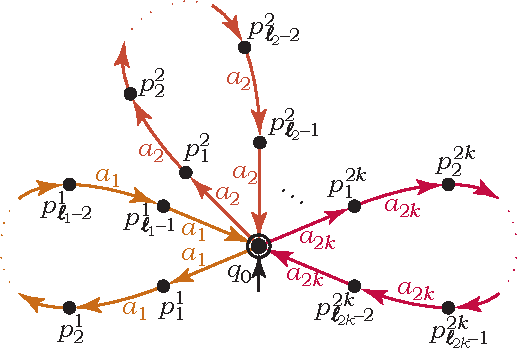
\includegraphics[scale=0.9]{rational_index_multi_A1}
	\caption{DFA $\mathcal{B}$ defined in Lemma~\ref{rational_index_multi_lower_bound_lemma} for $d=1$
		and fixed $k \geqslant 0$.}
	\label{mcfg_dim1_lower_aut}
\end{figure}

Consider the length of the shortest string in $w \in L(G) \cap L(\mathcal{B})$.
Every such string is of the form $a^i_1 \ldots a^i_{2k}$ for $i \geqslant 1$.
The automaton accepts the string of this form iff $i$ is a multiple of all lengths
of its cycles $\ell_1, \ldots, \ell_{2k}$. All lengths of the cycles are primes by 
construction, thus the least such $i$ is equal to $\prod\limits_{i=1}^{2k}\ell_i$.
Then the length of $w$ is estimated as follows.

\begin{equation*}
	|w|
		=
	2k\prod\limits_{i=1}^{2k} \ell_i
		> 
	2k \prod\limits_{i=1}^{2k} \frac{n}{4k}
		=
	2k \frac{n^{2k}}{(4k)^{2k}}
		=
	\frac{1}{k^{2k-1}\cdot 2^{4k-1}}
	n^{2k}
%		=
%	\frac{2k n^{2k}}{(4k)^{2k}} = \frac{n^{2k}}{2^{4k-1}k^{2k-1}}.
\end{equation*}

\textbf{Induction step:} $dim(G) = d$.
By the induction hypothesis, there exists a $k$-component grammar
$\hat{G}=(\widehat{\Sigma}, \widehat{N}, \ranksymb, \widehat{R}, \widehat{S})$
of tree dimension bounded by $d-1$
that satisfies the condition of the lemma.
A $k$-component grammar of tree dimension bounded by $d$ is then defined
over the alphabet $\Sigma = \widehat{\Sigma} \cup \{a, b, c_1, \ldots, c_{2k-1}\}$,
where $a, b, c_1, \ldots, c_{2k-1} \not\in \widehat{\Sigma}$.
The set of nonterminal symbols of new grammar is $N = \widehat{N} \cup \{S, A, C\}$,
where all nonterminal symbols from $\widehat{N}$ preserve their original rank,
while new nonterminals $A, C, S \not\in \widehat{N}$
have $\rank{S}=\rank{A}=1$ and $\rank{C}=k$.
The rules of the grammar $G$ include all rules from $\widehat{G}$ and the following additional rules.
\begin{align*}
	S(x_1 \ldots x_k) &\gets C(x_1, \ldots, x_k) \\
	C(yx_1c_1, c_2 x_2 c_3, \ldots, c_{2k-2}x_kc_{2k-1}) &\gets A(y), C(x_1, \ldots, x_k) \\
	C(y c_1, c_2 c_3, \ldots, c_{2k-2} c_{2k-1}) &\gets A(y) \\
%	C(x_0x_1c_1,\ldots, c_{2k-2}x_kc_{2k-1}) &\gets A(x_0), B(x_1, \ldots, x_k) \\
%	B(\varepsilon, \ldots, \varepsilon) &\gets \\
	A(ayb) &\gets A(y) \\
	A(ayb) &\gets \widehat{S}(y).
\end{align*}
Here, the nonterminal $A$ defines all substrings of the form $a^i u b^i$, where 
$i \geqslant 1$ and $u \in L(\widehat{G})$, as in the grammar from Lemma~\ref{rational_index_lower_bound_lemma}.
A nonterminal symbol $C$ generates all $k$-tuples of the form 
$(v_1 \ldots v_t c_1^t, c_2^t c_3^t, \ldots, c_{2k-2}^t c_{2k-1}^t)$, where 
$t \geqslant 1$ and $v_1, \ldots, v_t$ are strings defined by nonterminal $A$.
Finally, the nonterminal $S$ defines concatenations of all such $k$-tuples, so that the language 
generated by grammar $G$ is of the following form.

\begin{equation*}
	%L(G)=
	\set{a^{i_1} w_1 b^{i_1} \ldots a^{i_t} w_t b^{i_t} c_1^t \ldots c_{2k-1}^t}{t \geqslant 1, \:
		i_1, \ldots, i_t \geqslant 1, \:
		w_1, \ldots, w_t \in L(\widehat{G})}
\end{equation*}

Next it is claimed that the dimension of the grammar $G$ is at most $d$.
The dimension of every tree with the root labelled by a nonterminal $\widehat{S}$
is at most $d-1$, that is the maximal dimension of grammar $\widehat{G}$.

Then each subtree with the root labelled by $A$ has dimension bounded by $d-1$.
The dimension of subtrees with the root labelled by $C$ is at most $d$, because 
the lowest such subtree has the same dimension $d-1$ as subtree labelled by $A$,
and each next subtree has one child labelled by $A$ of dimension $d-1$ and one child $C$ of
dimension at most $d$.
The dimension of the root labelled by $S$ is equal to the dimension of the topmost
subtree labelled by nonterminal $C$, and, therefore, is at most $d$.

Let $n \geqslant 8 \cdot 2^d k^2 \ln 8k$ and $n$ be divisible by $2^dk$.
As $\frac{n}{2}$ is greater than $8 \cdot 2^{d-1} k^2 \ln 8k$ and is divisible by $2^{d-1}k$, 
by the induction hypothesis there exists an $\frac{n}{2}$-state automaton 
$\widehat{\mathcal{B}} = (\widehat{Q}, \widehat{\Sigma}, \widehat{\delta}, \widehat{q}_0, \{\widehat{q}_0\})$
 for grammar $\widehat{G}$ such that the length of the shortest string $\widehat{w}$ in the intersection
$L(\widehat{G}) \cap L(\widehat{\mathcal{B}})$ has the length at least 
$\frac{1}{k^{2k(d-1)-1} \cdot 2^{k(d-1)^2 + 5k(d-1) -2k -1}} n^{2k(d-1)}$.

Then $n$-state DFA $\mathcal{B} = (\Sigma, Q, q_0, \delta, \{q_0\})$
is constructed as follows. It consists of DFA $\widehat{\mathcal{B}}$ with 
at most $\frac{n}{2}$ states, and the second half of the states is used to 
construct cycles. Let $\ell_1, \ldots, \ell_{2k}$ be primes, such that 
$\frac{n}{8k} \leqslant \ell_i \leqslant \frac{n}{4k}$ for every $i$. 
These numbers define the lengths of the cycles, and the set of states of the new automaton
is as follows.

\begin{equation*}
	Q = \widehat{Q} \cup \{q_0,
		\underbrace{p^1_1, \ldots, p^1_{\ell_1-1}}_{\text{cycle by $c_1$}},
		\ldots,
		\underbrace{p^{2k-1}_1, \ldots, p^{2k-1}_{\ell_{2k-1}-1}}_{\text{cycle by $c_{2k-1}$}},
		\underbrace{q_1, \ldots, q_{\ell_{2k}-1}}_{\text{chain by $a$ and $b$}}\}
\end{equation*}
Overall, at most $2k \frac{n}{4k} = \frac{n}{2}$ states are used for constructing of cycles.

The transitions are similar to those in the proof of Lemma~\ref{rational_index_lower_bound_lemma},
with the only difference that instead of one cycle by $c$
the automaton in this proof has $2k-1$ cycles by $c_1$, \ldots, $c_{2k-1}$.
The initial state is $q_0$, it has a transition by $a$
to the initial state of $\widehat{\mathcal{B}}$,
continued by a transition by $b$ to $q_1$.
\begin{align*}
	\delta(q_0, a) &= \widehat{q}_0
		\\
	\delta(\widehat{q}_0, b) &= q_1
\intertext{%
A chain of transitions by $a$ and another chain by $b$
are as in Lemma~\ref{rational_index_lower_bound_lemma};
they use states from $q_1$ to $q_{\ell_{2k}-1}$.
}
	\delta(q_i, a) &= q_{i-1},
		&& \text{with } 1 \leqslant i \leqslant \ell_{2k}-1
		\\
	\delta(q_i, b) &= q_{i+1 \bmod \ell_{2k}},
		&& \text{with } 1 \leqslant i \leqslant \ell_{2k}-1
\intertext{%
For each $i$, with $1 \leqslant i \leqslant 2k-1$,
there is a cycle by $c_i$
in the states $q_0=p^i_0$, $p^i_1$, \ldots, $p^i_{\ell_i-1}$.
}
	\delta(p^i_j, c_i) &= p^i_{j+1 \bmod \ell_i},
		&& \text{with } 0 \leqslant j \leqslant \ell_i-1
\end{align*}
This automaton $\mathcal{B}$ is illustrated in Figure~\ref{dimautomatamcfg:generalized}.

\begin{figure}[t]
	\centering
	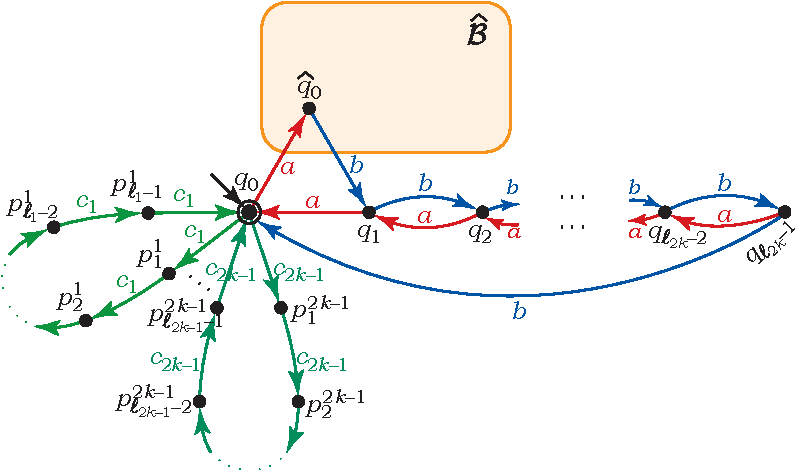
\includegraphics[scale=0.9]{rational_index_multi_Ad.pdf}
	\caption{DFA $\mathcal{B}$ defined in Lemma~\ref{rational_index_multi_lower_bound_lemma} for $d \geqslant 2$ and fixed $k$,
		which incorporates DFA $\widehat{\mathcal{B}}$ for $d-1$ and $k$.}
	\label{dimautomatamcfg:generalized}
\end{figure}

Every string $w$ in $L(G) \cap L(\mathcal{B})$
is of the form 
$w = a^{i_1} w_1 b^{i_1} \ldots a^{i_t} w_t b^{i_t} c_1^t \ldots c_{2k-1}^t$,
with $t \geqslant 1$,
$i_1, \ldots, i_t \geqslant 1$
and $w_1, \ldots, w_t \in L(\widehat{G})$,
because it is defined by $G$.
The string $w$ is also accepted by $\mathcal{B}$,
and, up to the first $c_1$, the automaton's computation proceeds
as in the proof of Lemma~\ref{rational_index_lower_bound_lemma}.

\begin{claim}
After reading each prefix $a^{i_1} w_1 b^{i_1} \cdots a^{i_s} w_s b^{i_s}$ of $w$,
with $s \in \{0, \ldots, t\}$,
the automaton comes to the state $q_{s \bmod \ell_{2k}}$.
\end{claim}

Thus, the automaton $\mathcal{B}$ reaches the first $c_1$ in the state $q_{t \bmod \ell_{2k}}$.
For the automaton to proceed further, this state must be $q_0$,
and hence $t$ is divisible by $\ell_{2k}$.
Next, the automaton reads each of the blocks $c_1^t$, \ldots, $c_{2k-1}^t$,
and must begin and end reading each of them in the same state $q_0$.
Therefore, $t$ must also be divisible by all numbers $\ell_1$, \ldots, $\ell_{2k-1}$.
As all $\ell_i$ are primes,
$t$ is divisible by their product $\prod\limits_{i=1}^{2k}\ell_i$.

As in the proof of Lemma~\ref{rational_index_lower_bound_lemma},
the automaton begins and ends reading each substring $w_i$
in the state $\widehat{q}_0$,
and hence all these strings are in $L(\widehat{G}) \cap L(\widehat{\mathcal{B}})$.

The shortest $w$ satisfying the above constraints
then has $t=\prod\limits_{i=1}^{2k}\ell_i$,
and its length is at least $t \cdot |\widehat{w}|$,
where $\widehat{w}$ is the shortest string in $L(\widehat{G})$.
Using a lower bound on $|\widehat{w}|$ given by the induction hypothesis,
the lower bound on the length of $w$ is estimated as follows.
\begin{multline*}
	|w|
		\geqslant
	\bigg(\prod\limits_{i=1}^{2k}\ell_i\bigg) \cdot |\widehat{w}|
		\geqslant \\ \geqslant
	\bigg(\prod\limits_{i=1}^{2k}\frac{n}{8k}\bigg) \cdot
	\frac{1}{k^{2k(d-1)-1} \cdot 2^{k(d-1)^2 + 5k(d-1) -2k -1}} \Big(\frac{n}{2}\Big)^{2k(d-1)}
		= \\ = %d^2 -2d + 1 + 3d -3 - 3 = d^2 + d - 5
	\frac{n^{2k}}{2^{6k}k^{2k}} \cdot 
	\frac{1}{k^{2kd-2k-1} \cdot 2^{k(d-1)^2 + 5k(d-1) -2k -1 + 2k(d-1)}} n^{2k(d-1)}
	= \\	= %d^2 + d - 5 + 4 + 2d - 2 = n^2 + 3d -3
	\frac{1}{k^{2kd-1} \cdot 2^{kd^2 + 5kd -2k -1}} n^{2kd}.
\end{multline*}
\qed
\end{proof}



\begin{theorem}\label{rational_index_multi_lower_bound_theorem}
For every $d \geqslant 1$, $k \geqslant 2$
there is a grammar $G$ of bounded tree dimension $d$,
such that for every $n \geqslant 8 \cdot 2^d k^2 \ln 8k$
there is an $n$-state partial DFA $\mathcal{B}$,
such that the shortest string $w$ in $L(G) \cap L(\mathcal{B})$
is of length at least
$\frac{k}{2^{kd^2 - kd -2k -1} \cdot (8k+1)^{2kd}} n^{2kd}$.
%$\Omega(n^{2kd})$.
\end{theorem}
\begin{proof}
%\es{Получилась очень страшная константа,}
%\es{если в неравенствах использовать $k \geqslant 2$, то будет симпатичнее}
Let $G$ be the grammar given for $d$ by Lemma~\ref{rational_index_multi_lower_bound_lemma}.
Let $2^d k r \leqslant n < 2^d k (r+1)$, for some integer $r$.
Then $r \geqslant 8k \ln 8k$
(for otherwise $n$ would be less than $8 \cdot 2^d k^2 \ln 8k$),
and $2^d k r \geqslant 2^{d+1} k$.

Since $2^d k r$ is divisible by $2^dk$
and is at least $8 \cdot 2^d k^2 \ln 8k$,
by Lemma~\ref{rational_index_multi_lower_bound_lemma},
there is a DFA $\mathcal{B}$ with $2^d k r \leqslant n$ states,
such that the length of the shortest string $w$ in $L(G) \cap L(\mathcal{B})$
is at least $\frac{1}{k^{2kd-1} \cdot 2^{kd^2 + 5kd -2k -1}} \cdot (2^d k r)^{2kd}$.
This is the desired $n$-state DFA.

%(r/(r+1) >= 2/3, 3r/2(r+1) >= 1)
%n < 2^d (r+1) <= 2^d (r+1) 3r/2(r+1) = 3/2 2^d r
%2/3n < 2^d r

Since $r > 8k$,
the inequality $n < 2^d k (r+1)$ implies that
$n < 2^d k r \frac{8k+1}{8k}$
and accordingly $2^d k r > n \frac{8k}{8k+1}$.
Then, the lower bound on the length of $w$
is expressed as a function of $n$ as follows.
%$n < 2^d k r\frac{8k \ln 8k}{8k \ln 8k -1}$,
%because $r+1$ is at most $\frac{8k \ln 8k}{8k \ln 8k -1}r$ for $r \geqslant 8k \ln 8k -1$.
%Then $2^d k r > \frac{8k \ln 8k - 1}{8k \ln 8k}n$,
\begin{align*}
	|w|
		&\geqslant 
	\frac{1}{k^{2kd-1} \cdot 2^{kd^2 + 5kd -2k -1}} (2^d k r)^{2kd}
		> \\ &>
	\frac{1}{k^{2kd-1} \cdot 2^{kd^2 + 5kd -2k -1}} \Big(n \cdot \frac{8k}{8k+1}\Big)^{2kd}
		= \\ &=
	\frac{1}{k^{2kd-1} \cdot 2^{kd^2 + 5kd -2k -1}} \cdot \frac{2^{6kd} \cdot k^{2kd}}{(8k+1)^{2kd}} \cdot n^{2kd}
		= \\ &=
	\frac{k}{2^{kd^2 - kd - 2k - 1} (8k+1)^{2kd}} \cdot n^{2kd}
\end{align*}
\qed
\end{proof}

The final conclusion on the rational index of $k$-component grammars with tree dimension bounded by $d$
is that it is in the worst case of the order $\Theta(n^{2kd})$.


\begin{comment}
Let $m = 2^dr = n - q$.
Then
\begin{align*}
	n > m > 2^{d+1} 
\\
   \frac{n}{2} > 2^d > q
\\
  (n-q)^{2d} \geqslant \left( \frac{n}{2}\right)^{2d}
\end{align*}
Consider an NFA $\widehat{\mathcal{B}}$ with $m = n - q = 2^d r$ states. By Lemma~\ref{rational_index_lower_bound_lemma} the shortest string $\widehat{w}$ in $L(G) \cap L(\mathcal{B})$
is of length at least $\frac{m^{2d}}{2^{d^2 + 3d - 3}} = \frac{(n-q)^{2d}}{2^{d^2 + 3d - 3}}$.

But $(n-q)^{2d} \geqslant \left( \frac{n}{2}\right)^{2d}$ and, therefore, $\frac{(n-q)^{2d}}{2^{d^2 + 3d - 3}} \geqslant\frac{(n)^{2d}}{2^{2d} \cdot 2^{d^2 + 3d - 3}} = \frac{(n)^{2d}}{2^{d^2 + 5d - 3}}$. \qed
\end{comment}






\section{Rational indices for some language families}\label{section_implications}

For a few families of grammars known in the literature,
the results of this paper imply some bounds on their rational index.

\paragraph{Superlinear languages.}
A grammar $G = (\Sigma, N, R, S)$ is \textit{superlinear} (Brzozowski~\cite{superlinear})
if its nonterminal symbols split into two classes, $N = N_{lin} \cup N_{nonlin}$,
where rules for each nonterminal $A \in N_{lin}$
are of the form $A \to uBv$ or $A \to w$, with $B \in N_{lin}$, $u,v,w \in \Sigma^*$,
while rules for a nontermial $A \in N_{nonlin}$
are of the form $A \to \alpha B \beta$, with $B \in N$ and $\alpha,\beta \in (\Sigma \cup N_{lin})^*$.
A language is \textit{superlinear} if it is generated by some superlinear grammar. 

\begin{corollary}
For every superlinear grammar $G$,
the rational index $\rho_{L(G)}$ is at most $O(n^4)$.
\end{corollary}
\begin{proof}
Parse trees in a superlinear grammar $G$ have dimension at most 2.
Then, by Theorem~\ref{rational_index_upper_bound_theorem},
the rational index $\rho_{L(G)}$ is bounded by $O(n^4)$.
\end{proof}

Turning to a lower bound, note that the grammar
constructed in Theorem~\ref{lower_bound_theorem} for $d=2$
is actually superlinear.

\begin{corollary}
There exists a superlinear grammar $G$
with rational index $\rho_{L(G)}(n) \geqslant \frac{1}{648} n^4$.
\end{corollary}






\paragraph{Bounded-oscillation languages.}
The notion of oscillation of runs in pushdown automata,
applicable to Turing machines with auxiliary pushdown tape,
was introduced by Wechsung~\cite{Wechsung}.
\emph{Languages with oscillation bounded by $k$}
are then a generalization of the linear languages
(as one-turn pushdown automata are those with oscillation bounded by $k=1$).

This family was later studied by Ganty and Valput~\cite{BoundOsc},
who introduced the corresponding notion of oscillation in parse trees of grammars.
%They introduce the notion of harmonics of well-nested sequence of brackets,
%and give two equivalent definitions
%one in terms for runs of nondeterministic pushdown automata (NPDA),
%and the other using grammars and their parse trees.
%
\begin{comment}
using a hierarchy of \textit{harmonics}.
Let $\bar{a}$ be a \textit{push}-move and $a$ be a \textit{pop}-move.
Then an NPDA run $r$ can be described by a well-nested sequence $\alpha(r)$ of symbols $\bar{a}$ and $a$.
Two positions $i<j$ form a \textit{matching pair}
if the corresponding $\bar{a}$ at the $i$-th position of the sequence
matches with $a$ at the $j$-th position.
For example, string $\bar{a}\bar{a}\bar{a}aa\bar{a}aa$
has the following set of matching pairs: $\{(1, 8), (2, 5), (3, 4), (6, 7)\}$
($\bar{a}(\bar{a}(\bar{a}a)a)(\bar{a}a)a$).

Harmonics are inductively defined as follows:
\begin{itemize}
\item
	order 0 harmonic $h_0$ is $\varepsilon$
\item
	$h_{(i+1)}$ harmonic is $\bar{a}h_ia\ \bar{a}h_ia$.
\end{itemize}
An NPDA run $r$ is \textit{$k$-oscillating}
if the harmonic of order $k$ is the greatest harmonic
that occurs in $r$ after removing zero or more matching pairs. 
\emph{Bounded-oscillation languages} are languages accepted by pushdown automata with all runs $k$-oscillating. 

The oscillation of a parse tree $t$ in a grammar $G$
%can be defined similarly to the oscillation of a PDA run.
Given a parse tree $t$, we define corresponding well-nested string $\alpha(t)$ inductively as follows:
\begin{itemize}
\item
	if $n$ is the root of $t$ then $\alpha(t) = \bar{a}\alpha(n)$
\item
	if $n$ is a leaf then $\alpha(n)=a$
\item
	if $n$ has $k$ children, then
	$\alpha(n) = a\underbrace{\bar{a}\ldots\bar{a}}_\text{$k$ times}\alpha(n_1)\ldots\alpha(n_k)$.
\end{itemize}

Moreover, given a PDA run $r$, there exists a corresponding parse tree $t$ with the same well-nested string $\alpha(t)=\alpha(r)$ 
and vice versa \cite{BoundOsc}. T
herefore, a language $L$ is of bounded oscillation if all parse trees in a corresponding context-free grammar have bounded oscillation.
\end{comment}
%
Among other results, they
prove that oscillation of a parse tree is closely related to its dimension.

\begin{lemma}[Ganty and Valput~\cite{BoundOsc}]\label{boscdim}
Let $G = (\Sigma, N, R, S)$ be a grammar in the Chomsky normal form,
and let $t$ be a parse tree in $G$.
Then, $\osc t - 1 \leqslant \dim t \leqslant 2\osc t$.
\end{lemma}

Thus, $k$-bounded-oscillation grammars have dimension of parse trees bounded by $2k$,
and Theorem~\ref{rational_index_upper_bound_theorem} gives the following upper bound on the rational index
of these languages.
\begin{corollary}
Let $L$ be a $k$-bounded-oscillation language.
Then $\rho_{L}(n) = O(n^{4k})$.
\end{corollary}


\paragraph{Linear (non-branching) multi-component grammars.}
A multi-component grammar is called \emph{linear}~\cite{Engelfriet1997},
or, alternatively, \emph{non-branching}~\cite{KANAZAWA2019104449}
if each rule has no more than $r$ occurrences of nonterminals in its body. 
A unary branching grammar is often called non-branching or 
linear.
\begin{corollary}
For every linear $k$-component grammar $G$,
the rational index $\rho_{L(G)}$ is at most $O(n^{2k})$.
\end{corollary}
\begin{proof}
Parse trees in a non-branching $k$-component grammar $G$ have dimension at most 1.
Then, by Theorem~\ref{rational_index_multi_upper_bound_theorem},
the rational index $\rho_{L(G)}$ is bounded by $O(n^{2k})$.
\end{proof}






\section{Adaptation to other grammar families?}\label{section_adaptation}

Roughly speaking, it was proved that if the branching of parse trees
in an ordinary (context-free) grammar is restricted,
then the rational index of the language is polynomial
of a certain degree that depends on the bound on the branching.
The result is generalized to multi-component grammars,
where the degree of the polynomial additionally depends on the rank of the grammar.
The question is, could this kind of results
hold for any other grammar families of interest,
under suitable restrictions on the structure of their parse trees?


\paragraph{LL($k$), LR($k$) and unambiguous grammars.}
LL($k$) grammars, LR($k$) grammars and unambiguous grammars
are classical subfamilies of grammars
that are notable for their beautiful theoretical properties
and diverse practical applications.
Under the restriction of $d$-bounded dimension of parse trees,
the rational index of all these grammars
is subject to the upper bound $O(n^{2d})$
given in Theorem~\ref{rational_index_upper_bound_theorem}.
It turns out that the lower bound $\Omega(n^{2d})$ holds as well,
because all grammars constructed in Theorem~\ref{lower_bound_theorem}
can be transformed to the most restricted of these subfamilies:
\emph{LL($1$)-grammars in the Greibach normal form},
also known as \emph{simple grammars}.

A grammar $G = (\Sigma, N, R, S)$ is LL(1) in the Greibach normal form
if every rule is of the form $A \to a \alpha$,
with $a \in \Sigma$ and $\alpha \in (\Sigma \cup N)^*$,
and if, furthermore, there is at most one such rule for every pair $(A, a)$.
Both grammars in the proof of Theorem~\ref{lower_bound_theorem}
can be rewritten as LL(1) grammars in the Greibach normal form:
the first language $\set{a^i b^i}{i \geqslant 1}$
is defined by a grammar with the rules
\begin{align*}
	S &\to a T \\
	T &\to a T b \ | \ b
\end{align*}
The second language
consists of all strings 
$a^{i_1} w_1 b^{i_1} \ldots a^{i_t} w_t b^{i_t} c^t$,
with $t \geqslant 1$,
$i_1, \ldots, i_t \geqslant 1$,
and with $w_1, \ldots, w_t$ defined by a nonterminal symbol $\widehat{S}$
using some rules that already satisfy the requirement of being LL(1) in the Greibach normal form.
This language is defined by the following grammar.
\begin{align*}
	S &\to a A T \\
	A &\to a A b \\
	A &\to \widehat{S} b
		&& (\widehat{S} \to \sigma \in \widehat{R}) \\
	T &\to c \ | \ a A T c
%	S &\to A S c \ | \ A c \\
%	A &\to a A b \ | \ a \widehat{S} b
\end{align*}
An interested reader can verify that the dimensions of parse trees
in the proof of Theorem~\ref{lower_bound_theorem}
are the same for this grammar,
and hence the argument remains valid with this grammar substituted.


\paragraph{Conjunctive and Boolean grammars.}
Conjunctive grammars are an extension of ordinary (context-free) grammars
with a conjunction operation,
so that each rule is of the form $A \to \alpha_1 \& \ldots \& \alpha_m$,
with $m \geqslant 1$ and $\alpha_1, \ldots, \alpha_m \in (\Sigma \cup N)^*$;
such a rule states that every string defined by each $\alpha_i$
is then defined by $A$.
Boolean grammars further extend the model with a conjunction operation.
These grammars preserve the notion of a parse tree,
which becomes an acyclic graph,
and are primarily notable for generalizations of classical parsing algorithms to handle these grammars.
An interested reader is referred to an up-to-date survey of conjunctive grammars~\cite{ConjunctiveTokyo}
and to an earlier survey of Boolean grammars~\cite{BooleanSurvey} for more details.

The question is, could any restriction on the structure of branching in parse trees for these grammars
lead to any upper bound on the rational index?
Unfortunately, no way of adapting the results of this paper to these models is anticipated.
Consider that the language of valid accepting computations of a Turing machine (VALC)
is an intersection of two linear languages;
a conjunctive grammar can define such an intersection
by including two linear grammars, with initial symbols $A$ and $B$,
and adding a rule $S \to A \& B$.
Parse trees in this grammar will have
the simplest possible structure for a conjunctive grammar,
with two linear trees coming out of the root,
and with each leaf shared between these two trees.
However, since checking the emptiness of VALC is undecidable,
there is no \emph{a priori} recursive upper bound on the rational index.


\begin{comment}
\section{Conclusion and open problems}\label{section_conclusion}

Languages of bounded tree dimension were proved to have polynomial rational index.
This implies, in particular,
that the CFL-reachability problem and Datalog query evaluation for these languages is in NC,
and the degree of the polynomial becomes a constant factor for the circuit depth.
%This class is a natural generalization of linear languages,
%and might be the largest class of queries among such generalizations that is known to be in NC.
\end{comment}

\begin{comment}
There is another family of languages which has polynomial rational index,
%but is incomparable with the languages of bounded tree dimension:
the \emph{one-counter languages}.
%For example, the Dyck language $D_1$ is a one-counter language,
%but not the language of bounded tree dimension for any $d$.
Their rational index is known to be $O(n^2)$~\cite{ChistikovCzerwinskiHofmanPilipczukWehar}.
Could this class be generalized in the same manner as linear languages,
preserving the polynomial order of the rational index?
One can consider the Polynomial Stack Lemma by Afrati et al.~\cite{ChainQ},
where some restriction on the PDA stack contents is given,
or investigate the properties of the substitution closure of the one-counter languages,
which is known to have polynomial rational index~\cite{RatBasic}. 
\end{comment}




%\section*{Acknowledgment}

%The authors are grateful to the anonymous reviewers
%for numerous helpful remarks and suggestions,
%and particularly for alerting the authors
%of the work by Chytil and Monien~\cite{ChytilMonien}.

%This research was supported by the Russian Science Foundation, grant \textnumero 18-11-00100.



\bibliographystyle{splncs04}
\bibliography{rational_index}

\end{document}
